% !TeX root = ../../main.tex


\section{井筒内铁屑运移及分布规律}
%20260704想法：仿真->实验->外推。这个研究属于“基础性研究”（与4.适用条件中“拓深技术理论及基础性研究”对应），界定了研究的性质——是基础理论研究，不是工程应用。目的是“揭示影响工具应用效果的主控因素”，对应5.1.2 ①的要求是“研究不同流速、粘度、井斜下的运移规律”，通过实验验证哪些参数是影响运移的“主控因素”（Re（实验已经证明）、井斜角的影响在全井筒模型实验中展示）。

在井下封隔器套铣作业过程中，将产生包含多种形态碎屑的混合物（见图\ref{fig:iron_shavings_sample}），其中，金属碎屑（尤其是铁屑）不仅可能导致筛管堵塞风险，还可能导致工具活动部件卡滞。经磨铣封隔器作业上返的碎屑样本分析表明，金属碎屑主要包含环状颗粒、块状颗粒及丝状颗粒三种形态。其中，丝状铁屑因其特有的几何特征，易通过旋转与缠绕作用形成网状结构，从而显著提升孔隙滞留概率。该类颗粒的高长径比特性不仅加剧了运移过程的复杂性，其各向异性运动模式及增大的比表面积更强化了流体拖曳力与壁面吸附效应，为油井金属碎屑对流动通道的动态阻塞机制提供了更真实的物理表征。基于上述特性分析，本研究选取丝状铁屑作为典型颗粒开展建模研究，具体模型及参数见图\ref{fig:iron_particle_comparison}和表\ref{tab:simulation_params}。

\begin{figure}[htbp]
    \centering
    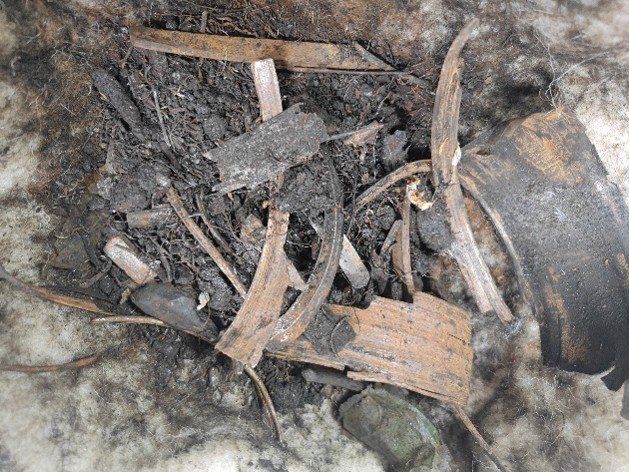
\includegraphics[width=0.5\textwidth]{figure/iron-shavings-sample.jpg}
    \caption{井下封隔器套铣作业中产生的金属碎屑样本}
    \label{fig:iron_shavings_sample}
\end{figure}

\begin{figure}[htbp]
    \centering
    % 子图 (a)
    \subfloat[实际铁屑颗粒]{%
        \begin{minipage}[t]{0.48\linewidth}
            \centering
            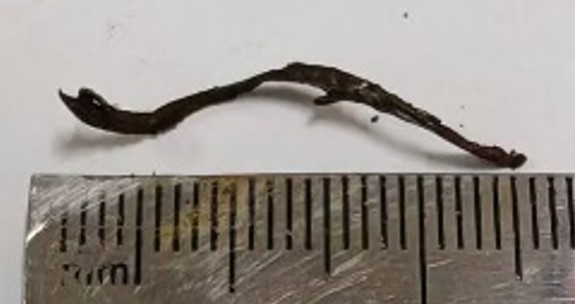
\includegraphics[width=\linewidth]{figure/iron-wire-actual.jpg}
            \label{fig:actual}
        \end{minipage}%
    }
    \hfill
    % 子图 (b)
    \subfloat[铁屑颗粒模型]{%
        \begin{minipage}[t]{0.45\linewidth}
            \centering
            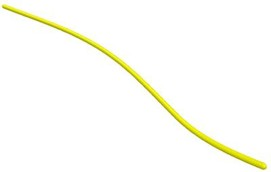
\includegraphics[width=\linewidth]{figure/iron-wire-model.jpg}
            \label{fig:model}
        \end{minipage}%
    }
    % 总标题
    \caption{铁屑颗粒及仿真模型}
    \label{fig:iron_particle_comparison}
\end{figure}

\begin{table}[htbp]
    \centering
    \caption{铁屑颗粒运移仿真参数}
    \label{tab:simulation_params}
    % 设置列格式：
    % c: 居中
    % p{width}: 固定宽度并自动换行（适合较长的中文名称）
    \begin{tabularx}{.9\textwidth}{CCCCC} 
        \toprule % 绘制顶部粗线
        % 表头部分
        序号 & 名称 & 符号 & 数值 & 单位 \\ 
        \midrule % 绘制中间细线
        
        % 数据行
        1 & 水平井筒长度 & $L$ & 1.5 & m \\
        2 & 井筒直径 & $D_H$ & 244.475 & mm \\
        3 & 钻杆直径 & $D_P$ & 88.9 & mm \\
        4 & 颗粒密度 & $\rho_p$ & 7800.0 & kg/m$^3$ \\
        5 & 洗井液密度 & $\rho_l$ & 1000.0、1300.0 & kg/m$^3$ \\
        6 & 井斜角 & $\theta$ & 0.0、45.0、90.0 & $^\circ$ \\
        7 & 洗井液入口流速 & $v_{in}$ & 0.17、0.27 & m/s \\
        8 & 洗井液粘度 & $\mu$ & 1.0、1.7 & mPa$\cdot$s \\
        9 & 沉积域距离井壁高度 & $H$ & 40.0 & mm \\
        10 & 颗粒与井壁静摩擦系数 & $\mu_s$ & 0.15 & - \\
        11 & 颗粒与井壁滑动摩擦系数 & $\mu_k$ & 0.1 & - \\
        
        \bottomrule % 绘制底部粗线
    \end{tabularx}
\end{table}

\subsection{洗井液粘度对铁屑运移规律的影响}
本节选取清水和氯化钠溶液（相对密度为1.3）两种洗井液进行对比。二者均可视为牛顿流体，但粘度不同，对铁屑颗粒的携带效果可能存在差异。在$\theta=90^\circ$、$v_{\mathrm{in}}=0.27\mathrm{m/s}$的条件下，通过仿真对比二者的携屑效果。图\ref{fig:iron_wire_distribution_viscosity}描述的是不同洗井液粘度下井筒内铁屑的分布情况（以颗粒速度着色）。从图中可以看出，洗井液粘度对铁屑颗粒运移效率的影响不大：随着洗井液粘度增大，移动铁屑床的速度略微增大，颗粒运移效率略有提高，出口处的铁屑颗粒有所增多。
%通过对不同洗井液的性能特点进行分析，可以为选择最适合的洗井液粘度提供参考，从而优化洗井操作并提高效率。

\begin{figure}[htbp]
    \centering
    % --- 子图 (a) ---
    % 使用 minipage 控制宽度，这里设为 0.9\textwidth 让图片大一点
    % [t] 表示顶部对齐，防止因为图片高度不同导致错位
    \subfloat[$\mu = 1.0\mathrm{mPa}\cdot\mathrm{s}$]{
        \begin{minipage}[t]{0.8\linewidth}
            \centering
            % 替换为你的第一张图片文件名
            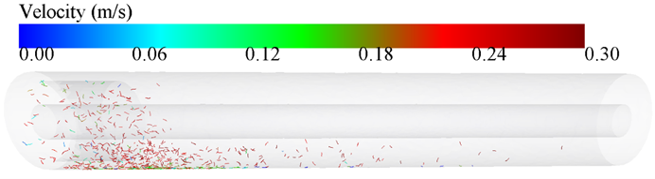
\includegraphics[width=\linewidth]{figure/iron-wire-distribution-1cp-velocity-colored.png} 
            \label{fig:viscosity_1.0}
        \end{minipage}
    }
    \vspace{0pt} % 上下两张图之间的垂直间距，可根据需要调整
    % --- 子图 (b) ---
    \subfloat[$\mu = 1.7\mathrm{mPa}\cdot\mathrm{s}$]{
        \begin{minipage}[t]{0.8\linewidth}
            \centering
            % 替换为你的第二张图片文件名
            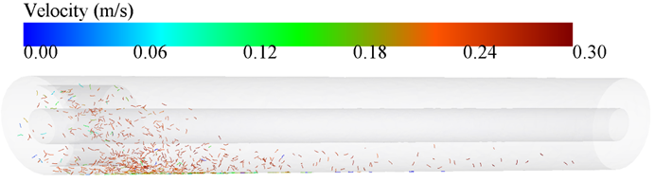
\includegraphics[width=\linewidth]{figure/iron-wire-distribution-1dot7-cp-velocity-colored.png} 
            \label{fig:viscosity_1.7}
        \end{minipage}
    }
    % --- 总标题 ---
    \caption{洗井液粘度对铁屑颗粒速度分布的影响（$\theta=90^\circ$,\ $v_{\mathrm{in}}=0.27\mathrm{m/s}$）}
    \label{fig:iron_wire_distribution_viscosity}
\end{figure}

图\ref{fig:iron_wire_mean_velocity_evolution_viscosity}为两种洗井液粘度下井筒稳态后铁屑颗粒沉积域铁屑颗粒运移速度图。从图中可以看出，$\mu$从$1.0\mathrm{mPa\cdot s}$增加到$1.7\mathrm{mPa\cdot s}$时，粘度增加到$1.7$倍，但铁屑的平均运移速度只增加到$1.04$倍，证明洗井液的粘度对铁屑运移的影响十分有限。
\begin{figure}[htbp]
    \centering
    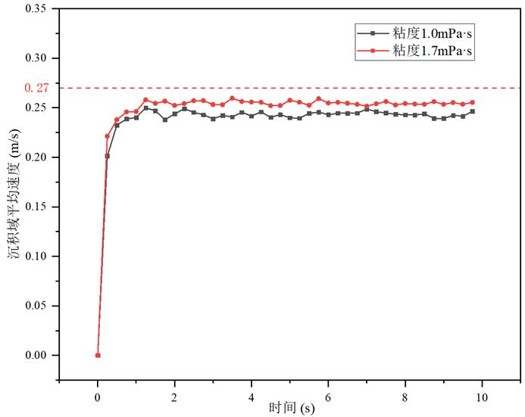
\includegraphics[width=0.7\textwidth]{figure/iron-wire-mean-velocity-evolution-viscosity.jpg}
    \caption{洗井液粘度对铁屑颗粒运移速度时间演变的影响（$\theta=90^\circ$,\ $v_{\mathrm{in}}=0.27\mathrm{m/s}$）}
    \label{fig:iron_wire_mean_velocity_evolution_viscosity}
\end{figure}

\subsection{洗井液流速对铁屑运移规律的影响}

本节探究洗井液流速对井筒环形空间内铁屑颗粒运移的影响。选取了水平段为研究对象，给定$\mu=1.7\mathrm{mPa\cdot s}$。

图\ref{fig:iron_wire_distribution_velocity}描述的是两种流速下井筒内铁屑颗粒分布情况，入口流速对铁屑颗粒运移行为的影响显著。铁屑的密度较大，在两种进口流速下，均表现出在边运移边沉积的现象，在水平管的底部位置有形成颗粒床的趋势。
随着洗井液流速的增加，从颗粒工厂出发的铁屑颗粒整体上产生了更大的轴向位移，颗粒整体的瞬时速度也有增加的趋势。这是由于洗井液流速增大时，铁屑颗粒受到流体沿轴向给予的拖拽力增加，铁屑颗粒沿轴向运移的速度增加。同时，增大的拖拽力也能对抗管壁摩擦效应，颗粒的运移效率增加。
\begin{figure}[htbp]
    \centering
    % --- 子图 (a) ---
    % 使用 minipage 控制宽度，这里设为 0.9\textwidth 让图片大一点
    % [t] 表示顶部对齐，防止因为图片高度不同导致错位
    \subfloat[$v_{\mathrm{in}} = 0.17\mathrm{m/s}$]{
        \begin{minipage}[t]{0.8\linewidth}
            \centering
            % 替换为你的第一张图片文件名
            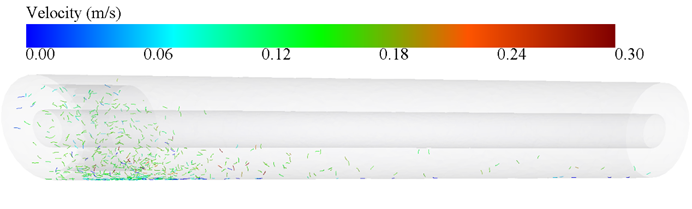
\includegraphics[width=\linewidth]{figure/iron-wire-distribution-1dot7cp-0dot17mpers.png} 
            \label{fig:distribution_velocity_0.17}
        \end{minipage}
    }
    \vspace{0pt} % 上下两张图之间的垂直间距，可根据需要调整
    % --- 子图 (b) ---
    \subfloat[$v_{\mathrm{in}} = 0.27\mathrm{m/s}$]{
        \begin{minipage}[t]{0.8\linewidth}
            \centering
            % 替换为你的第二张图片文件名
            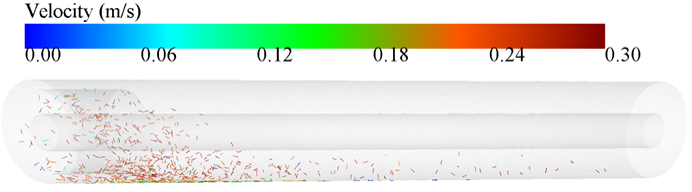
\includegraphics[width=\linewidth]{figure/iron-wire-distribution-1dot7cp-0dot27mpers.png} 
            \label{fig:distribution_velocity_0.27}
        \end{minipage}
    }
    % --- 总标题 ---
    \caption{洗井液流速对铁屑颗粒分布的影响（$\theta=90^\circ$,\ $\mu = 1.7\mathrm{mPa}\cdot\mathrm{s}$）}
    \label{fig:iron_wire_distribution_velocity}
\end{figure}

铁屑颗粒的运动迹线图直观地展现了颗粒的运动轨迹，本文选取了井筒内的部分铁屑颗粒，绘制了两种流速下其迹线图，如图\ref{fig:iron_wire_particle_track_velocity}所示。从图中可以看出，在颗粒工厂中产生的铁屑颗粒一经产生，将很快获得轴向移动速度，这一点可从左上至右下的迹线得到证明；且进口流速越大，迹线的斜率越小，颗粒获得的周向速度也越大。在两种情况下，颗粒落到管底后，以较大幅度弹跳的方式向前运动，而非形成密实的颗粒床以整体的形式运动。在图\ref{fig:distribution_velocity_0.27}中，铁屑颗粒在颗粒工厂右边界附近的迹线混叠密度也低于前者，说明进口流速提升时，颗粒得以弥散开来，颗粒床的形成受到了抑制。

%这两张图的总仿真时间是个很重要的变量。第一个总的仿真时间长，第二个总的仿真时间短。总仿真时间长，颗粒的运动轨迹就会更长，颗粒的运动轨迹就会更密集。总仿真时间短，颗粒的运动轨迹就会更短，颗粒的运动轨迹就会更稀疏。

\begin{figure}[htbp]
	\centering
	% --- 子图 (a) ---
	% 使用 minipage 控制宽度，这里设为 0.9\textwidth 让图片大一点
	% [t] 表示顶部对齐，防止因为图片高度不同导致错位
	\subfloat[$v_{\mathrm{in}} = 0.17\mathrm{m/s}$]{
		\begin{minipage}[t]{0.8\linewidth}
			\centering
			% 替换为你的第一张图片文件名
			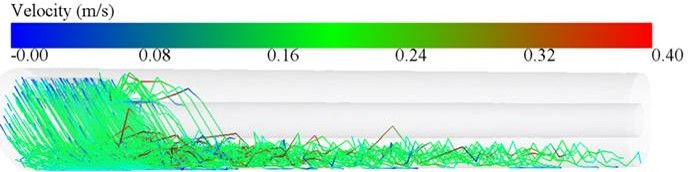
\includegraphics[width=\linewidth]{figure/iron-wire-particle-track-1dot7cp-0dot17mpers.jpg} 
			\label{fig:track_velocity_0.17}
		\end{minipage}
	}
	\vspace{0pt} % 上下两张图之间的垂直间距，可根据需要调整
	% --- 子图 (b) ---
	\subfloat[$v_{\mathrm{in}} = 0.27\mathrm{m/s}$]{
		\begin{minipage}[t]{0.8\linewidth}
			\centering
			% 替换为你的第二张图片文件名
			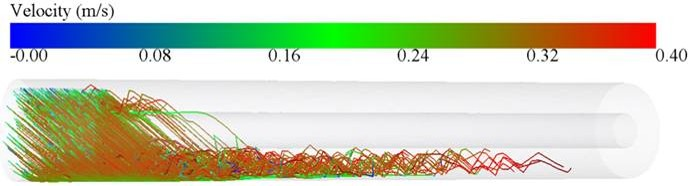
\includegraphics[width=\linewidth]{figure/iron-wire-particle-track-1dot7cp-0dot27mpers.jpg} 
			\label{fig:track_velocity_0.27}
		\end{minipage}
	}
	% --- 总标题 ---
	\caption{洗井液流速对铁屑颗粒分布的影响（$\theta=90^\circ$,\ $\mu = 1.7\mathrm{mPa}\cdot\mathrm{s}$）}
	\label{fig:iron_wire_particle_track_velocity}
\end{figure}

图\ref{fig:iron_wire_mean_velocity_evolution_incoming_velocity}给出了$v_{\mathrm{in}}=0.17\mathrm{m/s}$,\ $0.27\mathrm{m/s}$两种情况下铁屑颗粒在沉积域中运移速度定量结果。洗井液流动产生的携屑作用足以克服井筒内壁摩擦作用，沉积在井筒底部的铁屑形成移动铁屑床。颗粒的平均轴向运动速度是小于来流（平均）速度，这说明铁屑颗粒在井筒内的运移过程中，受到井壁摩擦力的影响。随着时间的推移，铁屑颗粒在沉积域中的平均运移速度逐渐趋于稳定，表明颗粒在井筒内的运移达到了动态平衡状态。随着洗井液流速的增加，井筒内沉积域铁屑颗粒运移速度也会大幅度增加，于是，洗井液的流速对铁屑运移有显著影响。
\begin{figure}[htbp]
	\centering
	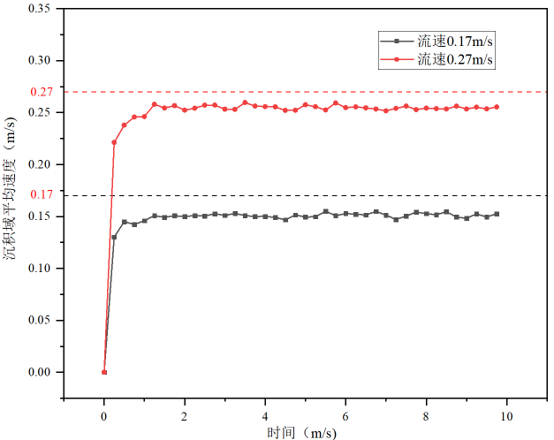
\includegraphics[width=0.7\textwidth]{figure/iron-wire-mean-velocity-evolution-incoming-velocity.png}
	\caption{洗井液速度对铁屑颗粒运移速度时间演变的影响（$\mu=1.7\mathrm{mPa\cdot s}$）}
	\label{fig:iron_wire_mean_velocity_evolution_incoming_velocity}
\end{figure}

\subsection{井斜对铁屑运移规律的影响}
本节将探究井斜对于井筒环形空间内铁屑颗粒运移的影响。选取了直井（$\theta = 0^\circ$）、45°斜井（$\theta = 45^\circ$）和水平井（$\theta = 90^\circ$）三种井斜，洗井液入口流速为$v_\mathrm{in}=0.27\mathrm{m/s}$，粘度取$\mu=1.7\mathrm{mPa\cdot s}$。

图\ref{fig:iron_wire_distribution_3angles}描述了不同井斜角度下井筒内铁屑颗粒瞬时分布情况。从图中可以看出，直井（$\theta = 0^\circ$）中井筒中铁屑不能向上迁移，目前的流体拖曳力不足以克服重力的作用。$\theta = 45^\circ$斜井中，铁屑床主要沉积在颗粒工厂附近的底部井壁上，距流体入口较近，流体出口附近几乎没有铁屑颗粒。$\theta = 90^\circ$的水平井，颗粒同样会聚集在井壁上，但颗粒床迁移的距离更远，聚集度更低，且出口处颗粒的数量比$\theta = 45^\circ$斜井中更多。
%$\theta = 45^\circ$和$\theta = 90^\circ$两种情况下，铁屑床都由移动床和静止床两部分组成，静止床的出现意味着上部铁屑积压，流体拖曳力、重力和摩擦作用相平衡；移动床的出现意味着流体的拖拽作用足以克服重力和管壁摩擦对单个铁屑颗粒的作用，使铁屑持续运移。表明，单个颗粒的行为有别于一群颗粒的行为，颗粒-颗粒之间的相互作用会影响颗粒的运移行为。
结合三种情况可以推测：第一，在直井中，作业产生的铁屑一定会下落至井底；第二，存在一个临界井斜$\theta_c$，当$\theta < \theta_c$时，铁屑颗粒会一直下落至井底形成堆积，而当$\theta > \theta_c$时，铁屑颗粒会在井筒壁面中形成堆积；第三，$\theta_c<45^\circ$，且其大小与流体的流速、粘度以及铁屑颗粒的密度、形状等因素相关。

\begin{figure}[htbp]
	\centering
	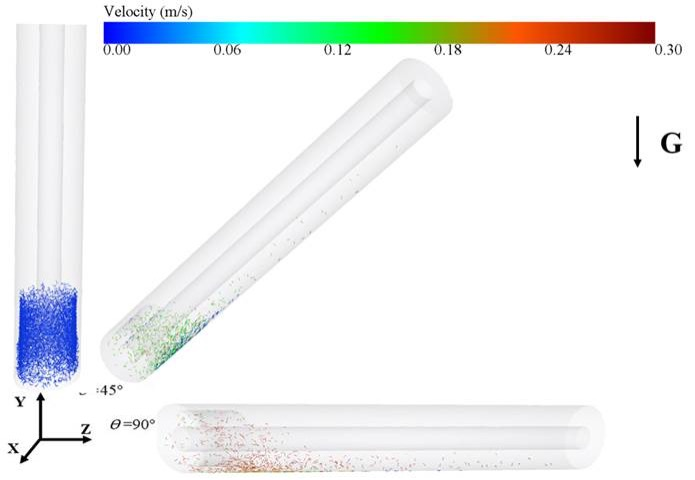
\includegraphics[width=0.7\textwidth]{figure/iron-wire-distribution-1dot7cp-0dot27mpers-3angles.jpg}
	\caption{井斜角对铁屑颗粒分布情况}
	\label{fig:iron_wire_distribution_3angles}
\end{figure}

铁屑颗粒的流动迹线图可以直观地描述颗粒的运动轨迹。首先选取井筒内的部分铁屑颗粒，绘制不同井斜角度下部分铁屑流动迹线图，如图\ref{fig:iron_wire_track_3angles}所示。直井（$0^\circ$）中铁屑运动轨迹平直，说明铁屑几乎不与井壁产生接触（或碰撞），短促的轨迹说明颗粒将向井底沉积，不能持续随流运移。各井斜条件下井壁处与颗粒工厂处的颗粒速度均较小，水平井环空内的颗粒速度大于斜井。这是由于井筒轴线与重力方向的夹角增大，环空中颗粒所受重力的影响愈发显著，颗粒在自身重力作用下下沉加快，洗井液在轴向上不足以提供足够的悬浮能量，颗粒堆积到底部后形成颗粒床，运移效率明显降低。

\begin{figure}[htbp]
	\centering
	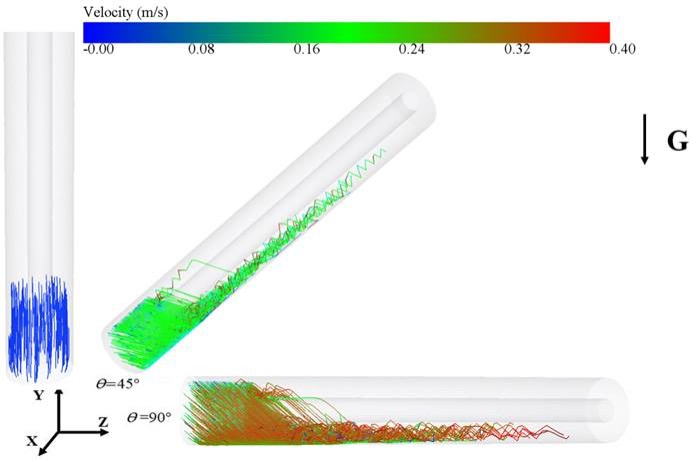
\includegraphics[width=0.7\textwidth]{figure/iron-wire-particle-track-1dot7cp-0dot27mpers-3angles.jpg}
	\caption{井斜角对铁屑运动轨迹的影响}
	\label{fig:iron_wire_track_3angles}
\end{figure}

斜井（$\theta = 45^\circ$）中移动铁屑床的平均运移速度小于水平井（$\theta = 90^\circ$），如图\ref{fig:iron_wire_velocity_3angles}所示。水平井中铁屑颗粒的运移速度接近环空平均流速，而斜井中铁屑颗粒的运移速度仅为环空平均流速的一半左右。

\begin{figure}[htbp]
	\centering
	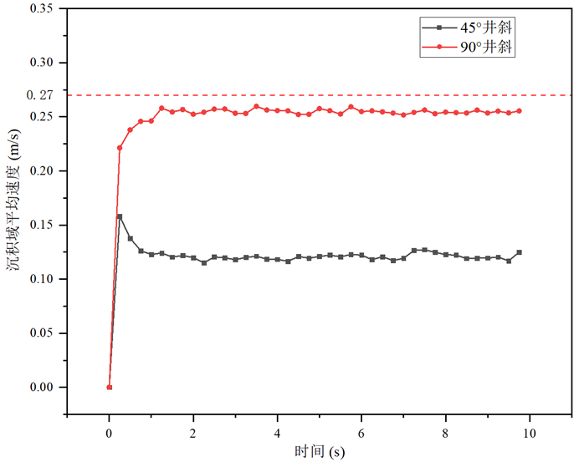
\includegraphics[width=0.7\textwidth]{figure/iron-wire-mean-velocity-evolution-3angles.png}
	\caption{井斜角对铁屑运动速度的影响}
	\label{fig:iron_wire_velocity_3angles}
\end{figure}

综合上述仿真结果可以发现，洗井液粘度增大和环空流速提高对铁屑颗粒的运移效率均有正向作用，因此选用更高粘度的洗井液、采用更大的洗井排量有助于铁屑颗粒从井筒中排出。但是，铁屑的运移行为受井筒倾角影响很大：在直井和小斜度井中，铁屑难以通过常规的洗井液循环方式排出，需开发具有\textbf{吸附}、\textbf{过滤}功能的\textbf{专用清洁工具}将铁屑从井筒中捞出。针对丝状铁屑的仿真结果可进一步推广至片状、块状铁屑等情形，此类高密度碎屑在井筒中的运移能力较差。

